\phantomsection
\chapter{Viola-Jones}

\noindent Viola-Jones algorithm is a visual object detection framework that is capable of processing images extremely rapidly while achieving high detection rates. It is based on a new image representation called "Integral Image" which allows the features used to be computed very quickly. It is also based on a learning algorithm, based on AdaBoost that gives extremely efficient classifiers. And it is also based on a method for combining classifiers in "cascade"; it allows to discard quickly the background of the image and to focus on the promising object-like regions \cite{VIO01}.
\newline

\phantomsection
\section{Haar features}

\vspace{\baselineskip}
\noindent The features used by Viola and Jones are called Haar features and are based on Haar wavelets. Haar wavelets are single wavelength square waves (one high interval and one low interval). In two dimensions, a square wave is a pair of adjacent rectangles: one light and one dark. The actual rectangle combinations used for visual object detection are not true Haar wavelets. Instead, they contain rectangle combinations better suited to visual recognition tasks. That is because of this difference that these features are called Haar features, or Haarlike features, rather than Haar wavelets \cite{HEW07}.
\newline

\noindent For example, the figure~\ref{haar_features_first_2_stage} shows the first two Haar features in the original Viola-Jones cascade \cite{HEW07}. These are all features from the original set of features. In figure~\ref{haar_features_extended}, there is an example of features from the extended set of features \cite{DIN08}. In the figure~\ref{haar_features_early_stage} , it is an example of a early stage in the Haar cascade. Each black and white patch represents a feature that the algorithm hunts for in the image \cite{HAR12}.
\newline

\begin{figure}[!h]
\begin{center}
\noindent 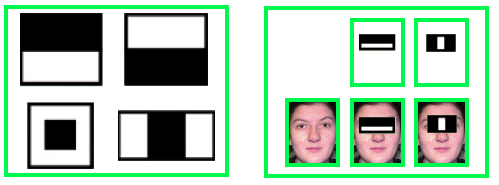
\includegraphics[scale=0.9]{figures/haar_features_first_2_stage} 
\newline
\caption{Example of the first two Haar features}
\label{haar_features_first_2_stage}
\end{center} 
\end{figure}

\begin{figure}[!h]
\begin{center}
\noindent 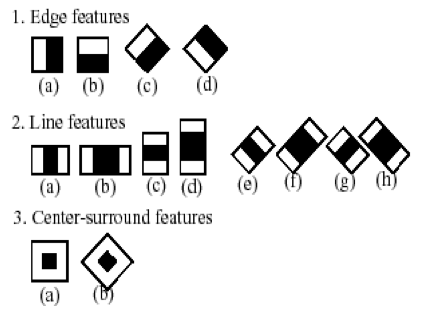
\includegraphics[scale=0.6]{figures/haar_features_extended} 
\newline
\caption{Extended set of features}
\label{haar_features_extended}
\end{center} 
\end{figure}

\begin{figure}[!h]
\begin{center}
\noindent 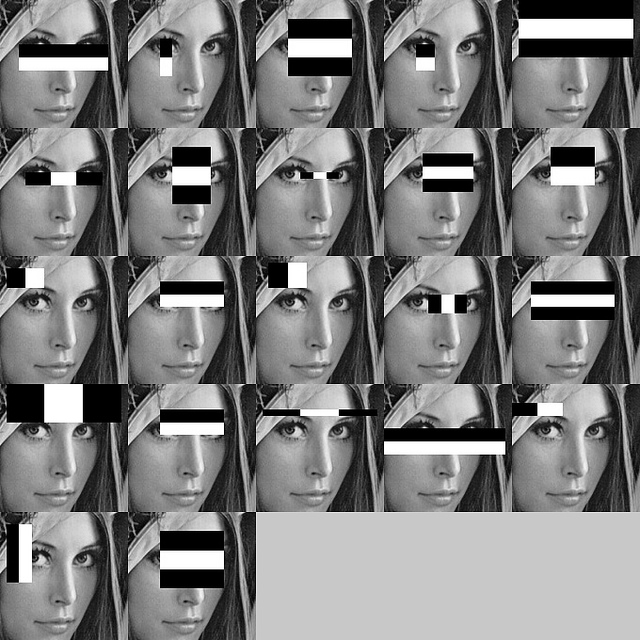
\includegraphics[scale=0.5]{figures/haar_features_early_stage} 
\newline
\caption{Example of an early stage in the Haar cascade}
\label{haar_features_early_stage}
\end{center} 
\end{figure}

\noindent The presence of a Haar feature is determined by subtracting the average dark-region pixel value from the average light-region pixel value. if the difference is above a threshold, that feature is said to be present and then it can go on to the next stage \cite{HEW07}. There is about 20-30 different stages. The first stage is a very coarse scan of the image. Stage 2 gets a little more detailed, stage 3 is a harder test to pass, stage 4 is even harder and it goes on and on. More it goes further into the cascade, more the features get increasingly complex and larger. It also takes more time to compute \cite{HAR12}.
\newline

\noindent For example, the figure~\ref{haar_feature_later_stage} shows the later stage in the Haar cascade where many more patterns of black and white rectangles need to match the candidate image \cite{HAR12}.
\newline

\begin{figure}[!h]
\begin{center}
\noindent 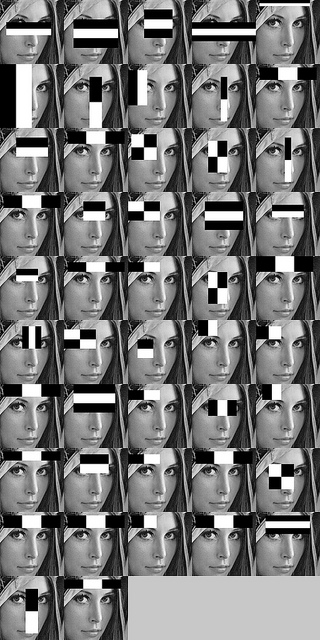
\includegraphics[scale=0.8]{figures/haar_feature_later_stage} 
\newline
\caption{Example of the later stage in the Haar cascade}
\label{haar_feature_later_stage}
\end{center} 
\end{figure}

\noindent Three kinds of feature are used by Viola and Jones. The value of a two-rectangle feature is the difference between the sum of the pixels within two rectangular regions. The regions have the same size and shape and are horizontally or vertically adjacent. A three-rectangle feature computes the sum within two outside rectangles subtracted from the sum in a center rectangle. Finally a four-rectangle feature computes the difference between diagonal pairs of rectangles \cite{VIO01}.
\newline

\noindent For example, the figure~\ref{haar_feature_description} shows the different kinds of rectangle features used by the Viola-Jones algorithm. Two-rectangle features are shown in (A) and (B). Figure (C) shows a three-rectangle feature, and (D) a four-rectangle feature \cite{VIO01}.
\newline

\begin{figure}[!h]
\begin{center}
\noindent 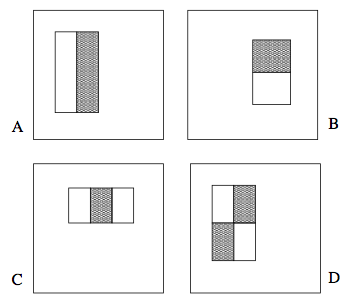
\includegraphics[scale=0.6]{figures/haar_feature_description} 
\newline
\caption{Example of the different kinds of rectangle features}
\label{haar_feature_description}
\end{center} 
\end{figure}

\noindent Rectangle features can be considered as somewhat primitive. In contrast with other features, rectangle features, while sensitive to the presence of edges, bars and other simple image structure, are quite coarse. It appears as though the set of rectangle features do however provide a rich image representation which supports effective learning. The extreme computational efficiency of rectangle features provides ample compensation for their limited flexibility \cite{VIO01}.
\newline

\phantomsection
\section{Integral image}

\vspace{\baselineskip}
\noindent Rectangle features can be computed very rapidly using an intermediate representation for the image which Viola and Jones called the "integral image" \cite{VIO01}. This integral image technique allows to determine the presence or absence of hundreds of Haar features at every image location and at several scales efficiently. In general, "integrating" means adding small units together; here, the small units are pixel values. The integral value for each pixel is the sum of all the pixels above it and to its left. Starting at the left and traversing to the right and down, the entire image can be integrated with a few integer operations per pixel \cite{HEW07}.
\newline

\noindent It means that the integral image, at location $ x,y $ contains the sum of the pixels above and to the left of $ x,y $, inclusive: \[ ii(x,y) = \sum_{x' \leq x,y' \leq y} i(x',y') \] where $ ii(x,y) $ is the integral image and $ i(x,y) $ is the regional image. In the figure~\ref{integral_image_description}, the value of the integral image at point $ (x,y) $ is the sum of all the pixels above and to the left \cite{VIO01}. 
\newline
	
\begin{figure}[!h]
\begin{center}
\noindent 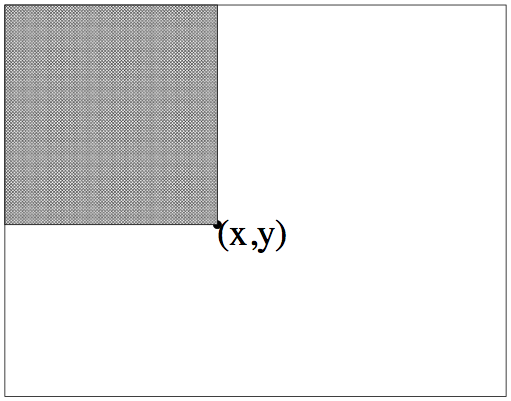
\includegraphics[scale=0.5]{figures/integral_image_description} 
\newline
\caption{Integral image}
\label{integral_image_description}
\end{center} 
\end{figure}
	
\noindent Using the following pair of recurrences: 
\begin{equation}
s(x,y) = s(x,y - 1) + i(x,y)
\end{equation}
\begin{equation}
ii(x,y) = ii(x - 1,y) + s(x,y)
\end{equation}
(where $ s(x,y) $ is the cumulative row sum, $ s(x,-1) = 0 $, and $ ii(-1,y) = 0 $) the integral image can be computed in one pass over the original image. Using the integral image any rectangular sum can be computed in four array references. In the figure~\ref{integral_image_four_array}, the sum of the pixels within rectangle D can be computed with four array references. The value of the integral image at location 1 is the sum of the pixels in rectangle $ A $. The value at location 2 is $ A + B $, a location 3 is $ A + C $, and at location 4 is $ A + B + C + D $. The sum within D can be computed as $ 4 + 1 - (2 + 3) $ \cite{VIO01}. 
\newline

\begin{figure}[!h]
\begin{center}
\noindent 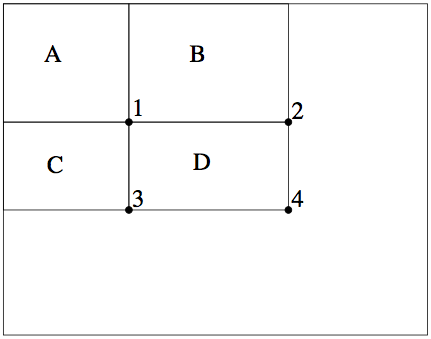
\includegraphics[scale=0.6]{figures/integral_image_four_array} 
\newline
\caption{Integral image with four array references}
\label{integral_image_four_array}
\end{center} 
\end{figure}

\noindent The integral is in fact the double integral of the image (first along rows and then along columns). The second derivative of the rectangle (first in row then in column) yields four delta functions at the corners of the rectangle \cite{VIO01}. 
\newline

\phantomsection
\section{Weak classifiers and AdaBoost}

\vspace{\baselineskip}
\noindent Features are extracted from a sub windows of a sample image. The base size for this sub window is 24 by 24 pixels. Each of all the features types are scaled and shifted across all possible combinations (In a 24 pixel by 24 pixel sub window, there are about 160,000 possible features to be calculated) \cite{SMY07}.
\newline

\noindent To select the specific Haar features to use, and to set threshold levels, Viola and Jones use a machine-learning method called AdaBoost. AdaBoost combines many "weak" classifiers to create one "strong" classifier. "Weak" here means that the classifier only gets the right answer a little more often than random guessing would. That is not very good. That is why a lot of weak classifiers are used. If a whole lot of these weak classifiers are used, and each one "pushed" the final answer a little bit in the right direction, this represents a strong, combined for to arrive at the correct solution. 
\newline

\noindent AdaBoost selects a set of weak classifiers to combine and assigns a weight to each (see figure~\ref{haar_feature_adaboost}). This weighted combination is the strong classifier \cite{HEW07}. The challenge is to associate a large weight with each good classification function and a smaller weight with poor functions. AdaBoost is an aggressive mechanism for selecting a small set of good classification functions which nevertheless have signficant variety \cite{VIO01}.
\newline

\begin{figure}[!h]
\begin{center}
\noindent 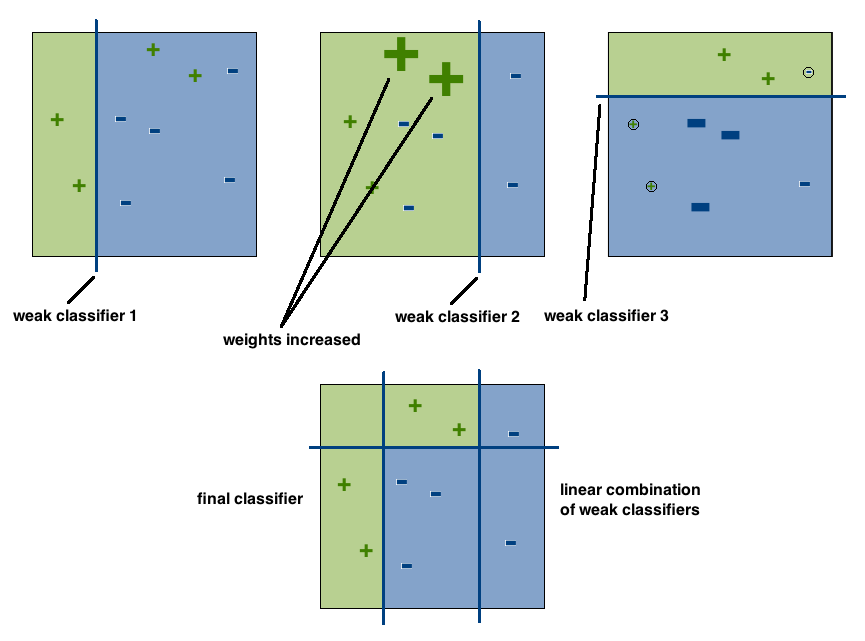
\includegraphics[scale=0.6]{figures/haar_feature_adaboost} 
\newline
\caption{AdaBoost method}
\label{haar_feature_adaboost}
\end{center} 
\end{figure}

\noindent Initial experiments demonstrated that a classifier constructed from 200 features using AdaBoost would yields reasonable results. Given a detection rate of 95\%, the classifier yielded a false positive rate of 1 in 14084 on a testing dataset (see figure~\ref{haar_feature_example_result})\cite{VIO01}.
\newline

\begin{figure}[!h]
\begin{center}
\noindent 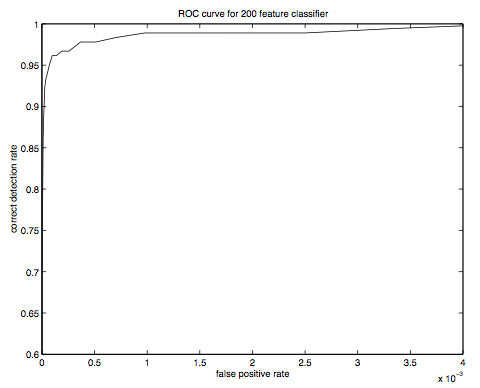
\includegraphics[scale=0.8]{figures/haar_feature_example_result} 
\newline
\caption{Receiver operating characteristic (ROC) curve for the 200 feature classifier}
\label{haar_feature_example_result}
\end{center} 
\end{figure}

\noindent The 200-feature classifier provides initial evidence that a boosted classifier constructed from rectangle features is an effective technique for object detection. In terms of detection, these results are compelling but not sufficient for many real-world tasks. In terms of computation, this classifier is probably faster than any other published system, requiring 0.7 seconds to scan an 384 by 288 pixel image. Unfortunately, the most straightforward technique for improving detection performance, adding features to the classifier, directly increases computation time \cite{VIO01}.
\newline

\phantomsection
\section{Classifiers cascade}

\vspace{\baselineskip}
\noindent Viola and Jones combined a series of AdaBoost classifiers as a filter chain, that is especially efficient for classifying image regions. Each filter is a separate AdaBoost classifier with fairly small number of weak classifiers. As in figure~\ref{haar_feature_cascade}, the classifier cascade is a chain of filters. Image subregions that make it through the entire cascade are classified as "Face". All others are classified as "Not Face" \cite{HEW07}.
\newline

\begin{figure}[!h]
\begin{center}
\noindent 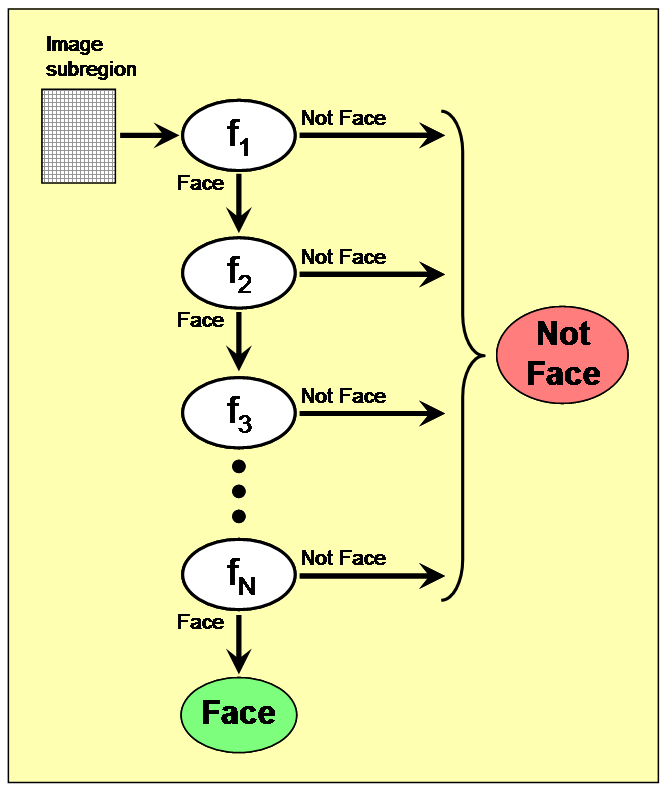
\includegraphics[scale=0.8]{figures/haar_feature_cascade} 
\newline
\caption{Classifiers cascade}
\label{haar_feature_cascade}
\end{center} 
\end{figure}

\noindent The acceptance threshold at each level is set low enough to pass all, or nearly all, face examples in the training set. The filters at each level are trained to classifiy training images that passed all previous stages. During use, if anyone of these filters fails to pass an image region, that region is immediately classified as "Not Face". When a filter passes an image region, it goes to the next filter in the chain. Image regions that pass through all filters in the chain are classified as "Face". Viola and Jones named this filtering chain a cascade \cite{HEW07}.
\newline

\noindent The order of filters in the cascade is based on the importance weighting that AdaBoost assigns. The more heavily weighted filters come first, to eliminate non-face image regions as quickly as possible. In figure~\ref{haar_feature_first_2_features}, it shows the first two features from the original Viola-Jones cascade superimposed on a face. The first one keys off the cheek area being lighter than the eye region. The second uses the fact that the bridge of the nose is lighter than the eyes \cite{HEW07}.
\newline

\begin{figure}[!h]
\begin{center}
\noindent 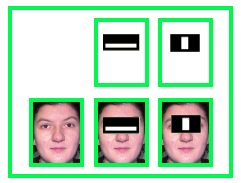
\includegraphics[scale=1]{figures/haar_feature_first_2_features} 
\newline
\caption{The first two Haar features in the original Viola-Jones cascade}
\label{haar_feature_first_2_features}
\end{center} 
\end{figure}

\phantomsection
\section{Test set and training}

\vspace{\baselineskip}
\noindent bla bla bla
\newline